\chapter{Background}\label{C:back}
Processing NMR relaxation in low SNR environments is crucial for dynamic environments such as well logging \cite{wellLoggingBook} \cite{UsingNMRPetrophysicalKenyon1992nuclear}. The current work done forms the benchmark to compare with the proposed technique of this project. This background survey details the current technique's performance. This establishes the evaluation criteria that will measure the proposed algorithm.

\section{NMR Relaxation}
Nuclear magnetic resonance involves determining the nature of the nuclei of a sample with their magnetic behaviour \cite{NMRSignalProcessingBook}. To provide an effective basis for the signal processing techniques to operate on, we start from examining the physics of the magnetism of the nuclei.

\subsubsection{Magnetism of the Nuclei}
The nucleus has two classical aspects that make it a microscopic magnet \cite{NMRSignalProcessingBook}:
\begin{enumerate}
    \item a nucleus has an electrical charge from the protons that make it up, and
    \item it may have a non-zero spin
\end{enumerate}
The spin creates magnetic dipole moment, $\vec{\mu}$. This phenomenon is expressed as the relation of angular momentum $\vec{J}$ and the gyro-magnetic ratio inherent to the nuclei, $\gamma$, such that

\begin{equation}
    \vec{\mu} = \gamma \vec{J}
    \label{eq:magneticMomentEquation}
\end{equation}
A macroscopic magnetic field formed by many nuclei, $\vec{M}$, is the summation over the total number of spins in the system, $N_s$  \cite{NMRSignalProcessingBook}.

\begin{equation}
    \vec{M} = \sum^{N_s}_{n = 1}\vec{\mu_{n}}
    \label{eq:macroMagnetic}
\end{equation}

Introducing a static magnetic field $B_0$ induces rotation of the magnetic moments of the nuclei. This rotation about $B_0$'s applied axis is called nuclear precession. The angular frequency of this rotation is known as the Larmor frequency  \cite{NMRSignalProcessingBook}. This is given by: 
\begin{equation}
    \omega_0 = \gamma B_0
    \label{ref:LarmorFreq}
\end{equation}
Holding the magnetic field $B_0$ constant means that all the same nuclei would exhibit nuclear precession at the same frequency. Their magnetic dipoles would precess at the same frequency.

In order to set all of the rotations of magnetic dipoles into phase we require another magnetic field, $B_1$. This field makes the system phase coherent  \cite{NMRSignalProcessingBook}. This is so that all of the magnetic dipoles of the same frequency constructively interfere, providing a strong enough signal to measure. $B_1$ is in the form of a short RF (radio frequency) pulse that lasts from microseconds to the milliseconds  \cite{NMRSignalProcessingBook}.

With phase coherence achieved there is a measurable macroscopic magnetic field from the nuclei. The change of this nuclei magnetic field is described by the Bloch equation  \cite{NMRSignalProcessingBook}:
\begin{equation}
    \frac{d\vec{M}}{dt} = \gamma \vec{M} \times \vec{B} - \frac{M_{x}\vec{i} + M_{y}\vec{j}}{T_2} - \frac{(M_z - M_{z}^0)\vec{k}}{T_1}
    \label{eq:blochEquation}
\end{equation}
where $\vec{M} = (M_x, M_y, M_z)$.
\subsubsection{Relaxation}

At the end of an RF pulse, the magnetic field $B_1$ is set to 0  \cite{NMRSignalProcessingBook}. In the rotating frame of reference this eliminates the first term of the Bloch equation. This results in the magnetism of the system of nuclei to be described by these two differential equations:
\begin{equation}
    \begin{cases}
          \frac{dM_{z'}}{dt}    =         -\frac{M_{z'} - M_{z}^0}{T_1}  \\
           \frac{dM_{x'y'}}{dt}    =         -\frac{M_{x'y'}}{T_2}  \\         
    \end{cases}
\end{equation}
The time evolution of the system is governed by these equations. Immediately after the RF pulse ($t = 0_+$) for the transverse magnetic field, $M_{x'y'}$, is expressed as:

\begin{equation}
    M_{x'y'}(t) = M_{x'y'}(0_+) e^{-t/T_2}
    \label{eq:T2ExpoenetialRelaxation}
\end{equation}

This exponential decay is referred to as the $T_2$ relaxation  \cite{NMRSignalProcessingBook}. The decay constant $T_2$ is used to give insight to the physical properties of the nuclei in the sample. This exponential model is only suitable for weak spin-spin systems such as fluids. Therefore, the analysis of the $T_2$ relaxation is limited to the behaviour of the fluids in a sample.

\subsubsection{Detecting Relaxation}
The resultant magnetic field can be detected by using Faraday's Law \cite{NMRSignalProcessingBook}:

\begin{equation}
    V(t) = -\frac{\partial \Phi(t)}{\partial t} = - \frac{\partial}{\partial t} \int_\text{object} \vec{B_r}(\bm{r}) \cdot \vec{M}(\bm{r} \cdot t) d \bm{r}
    \label{eq:detectionFaraday}
\end{equation}
After demodulation of the voltage \cite{NMRSignalProcessingBook}, we get a signal we can process and analyse:

\begin{equation}
    S(t) = \int_{\text{object}} M_{x,y}(\bm{r}, 0 )e^{i\gamma \Delta B(\bm{r})t} d \bm{r}
    \label{eq:detectionFinalSignal}
\end{equation}
The term $\Delta B $ varies in space due to the inhomogeneity of the magnetic field. This is a form of error introduced into the measurement process.

\subsection{The $T_2$ Density Function}
The density function of T2 relaxation times is referred to as $f(T_2)$. An example $T_2$ distribution is shown in figure \ref{fig:theModel}. The T2 density function forms the basis of analysis of fluids in a sample. There are two properties that relate the T2 relaxation to fluids in porous media: \textit{porosity}, and \textit{bound fluid fraction} \cite{NMRForRockskleinberg1993nuclear} \cite{wellLoggingBook}.

\begin{figure} [h]
    \centering
    \begin{subfigure}[b]{0.495\textwidth}
        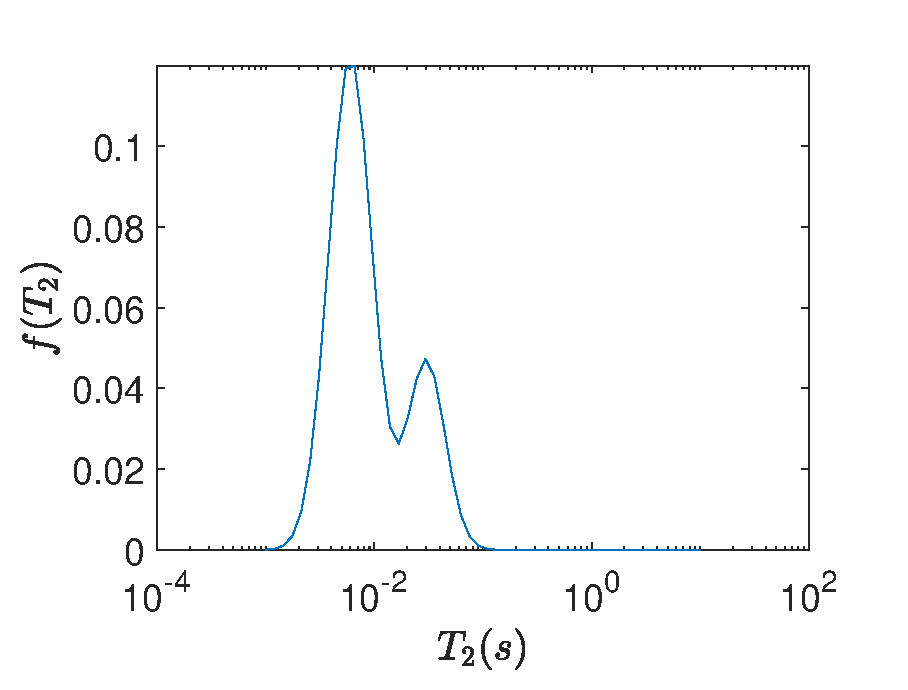
\includegraphics[width=\textwidth]{backgroundVector/densityFunction.eps}
        \subcaption{The density function $f(T_2)$}
        \label{fig:densityFunction}
    \end{subfigure}
    \begin{subfigure}[b]{0.495\textwidth}
        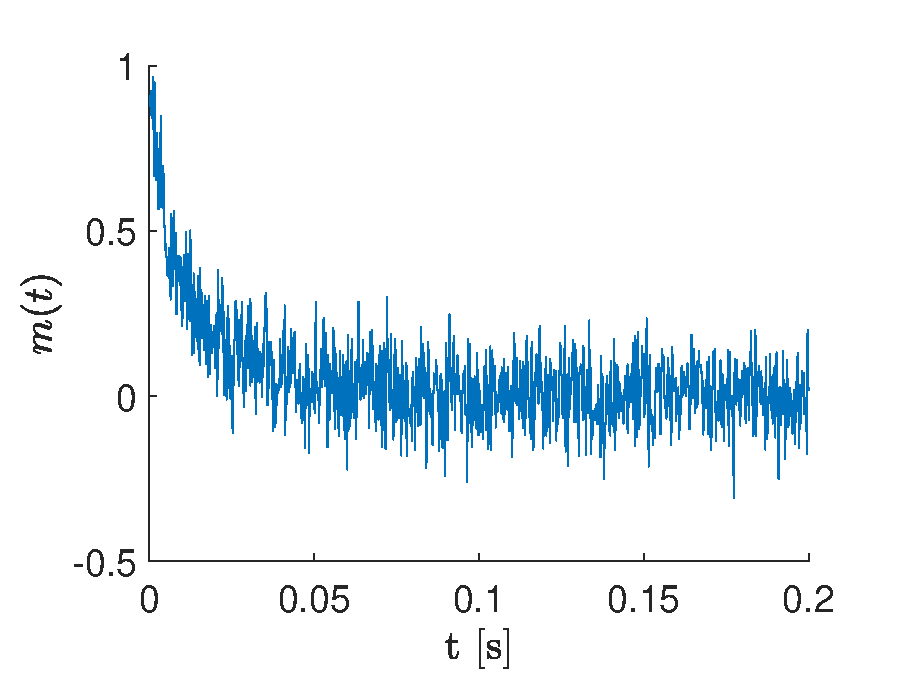
\includegraphics[width=\textwidth]{backgroundVector/measured.eps}
        \subcaption{The modelled measured data $m(t)$}
        \label{fig:measuredData}
    \end{subfigure}
    
    \caption{An example modelled $T_2$ density function and the measured data generated from it. It has unity porosity and a noise standard deviation of $\sigma_\epsilon = 0.2$}
    \label{fig:theModel}
\end{figure}

\subsubsection{Porosity}
The fraction of the rock volume that can be occupied by fluid is defined as the porosity ($\phi$) \cite{PorosityandT2Times}. After calibration with a water sample ($\phi = 1$), the integral over the entire density function is equal to the porosity.
\begin{equation}
    \phi = \int_0^\infty f(T_{2}) dT_{2}
\end{equation}
This is approximated to taking the sum over the discretised density function:
\begin{equation}
    \phi = \sum_i f(T_{2 i})
\end{equation}

\subsubsection{Bound Fluid Fraction}
Bound fluids are fluids that require significant capillary pressure to remove from porous media \cite{wellLoggingBook}. This pressure is caused by the fluid being placed in sufficiently small pores of the media. The volume of bound fluids - the bound fluid volume ($BFV$) \footnote{also known as the bulk fluid irreducible ($BVI$)} - is associated with relaxation times below a cut off value, $T_{2 \text{, cutoff}}$ \cite{wellLoggingBook}. This volume is obtained with:
\begin{equation}
    BFV = \int^{T_{2\text{, cutoff}}}_{T_{2\text{,min}}} f(T_2) d T_2
    \label{eq:boundFluidVolume}
\end{equation}
Free fluids conversely are fluids that are able to be extracted since they experience less capillary pressure restraining them \cite{NMRForRockskleinberg1993nuclear}\cite{BoundfluidFractionchen1998improving}. Therefore, the free fluid volume - also known as movable fluids ($BVM$) - can be expressed as the remaining fluid that is not bound in the T2 density function. Since the porosity is defined to be all of the fluid volume in the sample, the bound fluid fraction ($BFF$) can be expressed in terms of the porosity. 

The bound fluid fraction is expressed, where $T_{2\text{,min}} = 0$, as:
\begin{equation}
    BFF = 
    \frac{BFV}{BFV + BVM} =
    \frac{BFV}{\phi} = \frac{\int^{T_{2\text{, cutoff}}}_{0} f(T_2) d T_2}{\int_0^\infty f(T_{2}) dT_{2}}
    \label{eq:boundFluidFraction}
\end{equation}

\section{Inversion of Measured Data}
In order to compute the T2 relaxation times from the measured data we require a computational model that corroborates with the physical model. This model reveals that the measured data is ill-posed for an inversion problem.

\subsection{Model of T2 Relaxation Measurements}
The measured T2 relaxation of a sample can be modelled with the following integral
\begin{equation}
    m(t) = \int e^{\frac{-t}{T_2}} f(T_2) dT_2 + \epsilon
    \label{eq:T2RelaxationModelContinuous}
\end{equation}
As we are unable to numerically compute continuous functions, we discretise this into
\begin{equation}
    \hat{m}(t) = \sum^{N_y}_{k = 1} f_k e^{\frac{-t}{T_{2_k}}} + \epsilon
    \label{eq:T2RelaxationModel}
\end{equation}
This model corresponds with the detected exponential decay of the transverse magnetic field in eq. \ref{eq:T2ExpoenetialRelaxation}. The measurement data $m$ is made up of $N_2$ discrete measurements. The time constants of these exponential functions -$T_{2_k}$ - make up the T2 relaxation times. In the model itself: $N_y$ is the total number of relaxation times modelled, $f_k$ is the contribution of each exponential, and $\epsilon$ is the additive white Gaussian noise introduced by the measurement process.

Since we know the measurements are made of exponentially decaying functions, we can construct a kernel matrix, $K$, that maps from the T2 domain to the time domain. The T2 density function is modelled as a vector $f$. The measurement process is modelled by:
\begin{equation}
    m = Kf + \epsilon
    \label{eq:T2RelaxationModelMatrices}
\end{equation}


\subsection{Ill-posed Nature}
The goal of this project is to find the bound fluid fraction. This has traditionally required estimating $f$ and then computing from there. Transforming a \textit{noiseless} single exponential to an easily quantifiable time constant can be achieved with the Inverse Laplace Transform (ILT) \cite{BulterReedsDawsonMethod1981}.
\begin{equation}
   f_k\delta   \bigg(   \frac{1}{T_{2}} - \frac{1}{T_{2_k}} \bigg) = \mathcal{L}^{-1} \bigg\{ f_k e^{\frac{-t}{T_{2_k}}} \bigg\}
    \label{eq:InverseLaplaceNaive}
\end{equation}
The ILT is not suited for the noisy model due to the noise present in the measurements. There can be very different results for the same measured sample due to the random effect of noise. Also, the kernel matrix $K$ is very poorly conditioned for computation \cite{NumericalFredholm1971hanson1971numerical}. The measured signal cannot be frequency filtered since that process does not discriminate between the noise or the true signal. This necessitates the implementation of a numerical approximation of the inversion.

\section{The ILT (Inverse Laplace Transform) Technique}
The numerical inversion is based on the goal of minimising the difference between the true unknown distribution and the estimated distribution. The most popular technique is that described by Venkataramanan et al for one dimensional and two dimensional distributions \cite{Venk2DFredholm2002} \footnote{The ILT technique explored here is technically known as solving Fredholm integrals of the first kind}. This technique requires knowing the standard deviation of the noise present ($\sigma_\epsilon$).


\subsection{Inversion With Optimisation}
The Bulter-Reeds-Dawson (BRD) method \cite{BulterReedsDawsonMethod1981} provides the established technique for numerical computation of the ILT. This is an optimisation framework expressed as:
    
\begin{equation}
    \Phi(f) = \min_{f\geq0}  ||Kf_\alpha - m||^2 + \alpha||f_{\alpha}||^2
    \label{eq:minimseError1981Optimise}
\end{equation}    
In this framework we can see that the main cost being minimised is the difference between the hypothesised noiseless time domain data $Kf_\alpha$ and the actual measured data $m$. However, constricting the problem simply to just this allows for overfitting to the noise itself. To counteract this, the second term $\alpha||f_{\alpha}||^2$ is added to penalise the complexity of the hypothesised solution. This `smooths' the hypothesised $f$ to prevent it fitting to the noise \cite{RegularizationElden1977algorithms}. This process is known as \textit{regularisation}.
The BRD method \cite{BulterReedsDawsonMethod1981} sets the optimal regularisation parameter as
\begin{equation}
    \alpha_{\text{opt}} =  \frac{N_y \sqrt{ \sigma_{\epsilon} } }{||c||} 
    \text{, }
    \label{eq:optAlphaOptimise}
\end{equation} 
where the vector $c$ determines by the estimated density function $f_\alpha$ \cite{Venk2DFredholm2002} such that
\begin{equation}
    c =\frac {Kf_{\alpha} - m}{-\alpha}  
    \label{eq:optCOptimise}
\end{equation}  
    This method involves updating $c$ with $\alpha_{\text{opt}}$ and then computing $\alpha_{\text{opt}}$ for the new $c$ (fig. \ref{fig:2002Optimisation}). This iterative computation converges towards the density function we are trying to predict after approximately 20 iterations. The problem is convex \cite{BulterReedsDawsonMethod1981}, so the starting $\alpha$ and $c$ can be set to any value as it will automatically converge to the best answer. 

\begin{figure}[ht!]
    \centering
    \includegraphics[width=\textwidth]{BlockDiagram2002Optimisation.png}
    \caption{Computational work flow of the optimisation framework in the inverse Laplace transform}
    \label{fig:2002Optimisation}
\end{figure}

\subsection{Calculating $c$}
    Computing the $c$ vector can be computationally dangerous due to potential error introduced by the approximate inversion of a possibly ill behaved matrix \cite{BulterReedsDawsonMethod1981}. Therefore, computing the $c$ vector involves taking the dot product of $m$ with a positive semi-definite matrix 
 
\begin{equation}
    H = \text{step}(K'c)I \text{, where} \quad \text{step}(t) = 
    \begin{cases}
    1  & t \geq 0\\
    0  & t < 0
    \end{cases}
    \label{eq:makeSemiPostiveDefinite}
\end{equation}   
that feeds in the regularisation coefficient \cite{BulterReedsDawsonMethod1981} $\alpha$ in the form of
\begin{equation}
    c =  (KHK' + \alpha I)^{-1} m  
    \label{eq:optFindC}
\end{equation} 


\subsection{Measurement Data Compression} \label{section:compression}
To reduce computation time, the truncated singular value decomposition of the kernel is used \cite{Venk2DFredholm2002}. Starting with the singular value decomposition $K = U S V'$:
\begin{itemize}
    \item the first $n$ columns $\hat{U}$ and $\hat{V}$ are kept from $U$ and $V$, and
    \item the first $n$ columns and rows of $\hat{S}$ are kept from S \cite{TSVDHansen1987truncatedsvd}.
\end{itemize}

\begin{equation}
    \hat{K} = \hat{S} \hat{V}'
    \label{eq:compressedKernel}
\end{equation}
\begin{equation}
    \hat{m} = m' \hat{U}
    \label{eq:compressedMeasurement}    
\end{equation}

These are then used to make a new kernel and measurement vector. Here, the dimensionality is reduced from $N_2$ (thousands) dimensions to $n$ dimensions   (eq. \ref{eq:compressedMeasurement}, \ref{eq:compressedKernel}). The optimisation problem remains unchanged as $||K||^2 = ||USV'||^2 \approx ||SV'||^2$; we are minimising the same error. This holds because the singular values of $K$ decay very rapidly as it is an exponential kernel \cite{NumericalInversionLaplaceTransform1978}.



\section{The ILT+ Technique}
More recent techniques have built further on this optimisation approach by implementing extra constraints. These come in the form of more prior information used to compensate for the high noise environment of the measured data \cite{GruberT2Estimation2013}. This involves calculating aspects that are intrinsic to the T2 density function. These are known as linear functionals. The two main functionals used for this improved optimisation framework are \textit{moments} and \textit{tapered areas} (fig. \ref{fig:2013ILTXOptimisation}) \cite{GruberT2Estimation2013}.


\begin{figure}[ht!]
    \centering
    \includegraphics[width=0.9\textwidth]{ILTXBlockDiagram.png}
    \caption{Computational work flow of the optimisation framework for the ILT+ method.}
    \label{fig:2013ILTXOptimisation}
\end{figure}

\subsection{Estimation of Moments}
A moment is a description of the `weight' of the density function on the T2 axis \cite{VenkMellin2010}. An example of a moment is the first moment, the mean. The $\omega^{\text{th}}$ moment is defined as:

\begin{equation}
    \langle T_2^{\omega}  \rangle \equiv
    \frac
    {\int_{0}^{\infty}  T_2^{\omega} f_{T_2}(T_2)dT_2}
    {\int_{0}^{\infty}  f_{T_2}(T_2)dT_2 }
    =     
    \frac
    {\int_{0}^{\infty}  T_2^{\omega} f_{T_2}(T_2)dT_2}
    {\phi}
    \label{eq:defnMoment}
\end{equation}
The ILT+ requires an estimation of the moment directly from the measured data without knowledge of the density function. This estimation is implemented using the Mellin transform (MT) \cite{VenkMellin2010}:

\begin{equation}
\langle \hat{T_2^{\omega}}  \rangle =
\begin{cases}
        \frac{-1}{\Gamma (\mu) \phi}
        \int_{0}^{\infty}t^{\omega -1}[M(t) - \phi]dt &
        \text{ $-1<\omega<0$,}\\
        1 & \text{ $\omega=0$,}\\
        \frac{1}{\Gamma (\mu) \phi}
        \int_{0}^{\infty}t^{\omega -1}M(t)dt &
        \text{ $\omega>0$,}\\
\end{cases}
\label{eq:mellinTransform}
\end{equation}

The computed moment is a numerical value describing the density function. This has a propagated uncertainty that can be used to evaluate how much we should depend on it for the optimisation framework.


\subsection{Estimation of Tapered Areas}
Tapered areas are weighted areas under a T2 distribution \cite{TaperedAreaskleinberg1997tapered}. This is another linear functional that can be directly estimated from the measured data \cite{GruberLinearFunctionals2013}.

Tapered areas are computed directly from a density function by the use of a tapered step function. The specific transform used by Gruber et al is the Exponential Haar Transform (EHT) \cite{GruberLinearFunctionals2013}. This is defined in the $T_2$ domain as:

\begin{equation}
    K_a(T_2, T_c) = \frac{C}{\gamma}\tanh(\alpha \gamma) 
    \label{eq:expHaarTransformT2}
\end{equation}
The EHT is also defined in the time domain as:
\begin{equation}
    k_a(t, T_c) = C(-1)^n e^{\beta t} \text{, } \quad 2n\alpha < t < 2(n+1)\alpha \text{,}   \quad n \in \mathbb{Z}
    \label{eq:expHaarTransformTime}
\end{equation}
The actual tapered area ($B$) and the estimated tapered area ($\hat{B}$) are computed with an inner product of the EHT kernel and the data for their respective domains:

\begin{equation}
   \label{eq:estTaperedAreas}
   B = K_a(T_2,T_c)f(T_2),  \quad \hat{B} = k_a(t, T_c)m(t)
\end{equation}
The transform in the $T_2$ domain is normalised so that $T_2 = T_c$, $K = 0.5$ \cite{GruberLinearFunctionals2013}. To meet this property, the constants are set to be:
\begin{equation}
    C = \frac{0.7213}{T_c} \text{, } \quad \alpha = (1.572)T_c \text{, } \quad
   \beta = \frac{0.4087}{T_c}  \text{, } \quad \gamma = \frac{1}{T_2} + \beta  
   \label{eq:haarTransformConstants}
\end{equation}



\subsection{Constrained Optimisation}
    Directly estimated linear functionals are introduced as extra optimisation constraints to evaluate the accuracy of the estimated density function \cite{GruberT2Estimation2013}. These estimated functionals are also more accurate than simply using the ILT method \cite{GruberLinearFunctionals2013}. Therefore, the additional prior information yields a more accurate estimation of the density function in a low SNR environment. This forms the basis for the ILT+ method \cite{GruberT2Estimation2013}. The optimisation framework that aims to minimise the cost $Q(f_\alpha)$ takes the form of:
\begin{equation}
    Q(f_\alpha) = \min_{f\geq0}  ||W(Lf_\alpha - g)||^2 + \alpha||f_\alpha||^2
    \label{eq:2013Optimise}    
\end{equation}
    This framework is adapted from the ILT method (eq. \ref{eq:minimseError1981Optimise}) by appending the estimations and uncertainties of the tapered areas and moments onto the framework \cite{GruberT2Estimation2013} such that:
 \begin{equation}
    g = 
    \begin{bmatrix}
    m  \\
    \langle T_2^{\omega_1} \rangle \\
    \vdots \\
    \langle T_2^{\omega_{N_{m}}} \rangle \\
    B_1 \\
    \vdots \\
    B_{N_{a}}
    \end{bmatrix}
    \text{, } \quad
    L = 
    \begin{bmatrix}
    K  \\
    \frac{1}{\phi}T_{2}^{\omega_1}\\
    \vdots \\
    \frac{1}{\phi}T_{2}^{\omega_{N_{m}}}\\    
    K_{a}(T_2,T_{c_{1}}) \\
    \vdots \\
    K_{a}(T_2,T_{c_{3}})     
    \end{bmatrix}
    \text{, } \quad
    W = 
    \begin{bmatrix}
    \frac{1}{\sigma_\epsilon}  \\
    \frac{1}{\sigma_{\omega_1}}  \\ 
    \vdots \\
    \frac{1}{\sigma_{\omega_{N_{m}}}} \\
    \frac{1}{\sigma_B}\\
    \vdots\\
    \frac{1}{\sigma_{B_{N_{a}}}}
    \end{bmatrix}
    I
    \label{eq:2013NewOptVectors}  
\end{equation}    

\paragraph{}
    The $g$ vector contains $N_{m}$ estimated moments and $N_{a}$ estimated tapered areas. The $L$ matrix maps from the T2 domain to the time domain: the estimated density function ($f$), estimated moments of $f$, and estimated tapered areas of $f$. The $W$ matrix is a diagonal matrix that changes the weight of each respective value of $g$ and $L$ with division by their respective uncertainty. Therefore, the larger weight value we have, the more certain we are that the estimation is correct. The $m$ vector is compressed via the methodology detailed in section \ref{section:compression}. The compression is to the same degree as the ILT method. 

\paragraph{}
This review details the main techniques in the literature. The following section evaluates these techniques to form the benchmark for the proposed technique.





